\documentclass[a4paper,12pt, hidelinks]{report}

\usepackage{alltt, fancyvrb, url}
\usepackage{authblk}
\usepackage{graphicx}
\usepackage{subfigure}
\usepackage{wrapfig}
\usepackage{algorithmic}
\usepackage[utf8]{inputenc}
\usepackage{fontenc}
\usepackage{amsmath,stmaryrd,mathtools,algorithm}
\usepackage{amssymb}
\usepackage[document]{ragged2e}
\usepackage[italian]{babel}
\usepackage{hyperref}

\title{\Huge \textbf{Relazione Progetto OOP}}

\author{Giulianini Andrea, Lombardi Alessandro, Meluzzi Marco, Stockman Alessandro}
\date{\today}


\begin{document}

\maketitle
\justify

\tableofcontents

\chapter{Analisi}

\section{Requisiti}

Il programma qbert è un remake del videogioco arcade Q*Bert pubblicato nel 1982 dalla Gottlieb. In altri termini si tratta di un rifacimento che  tende a ricostruire abbastanza  fedelmente, se non tutte, almeno le principali caratteristiche del gioco originale.

\subsubsection{Requisiti funzionali}
\begin{itemize}
	\item Il giocatore servendosi degli appositi input da tastiera, può muovere il personaggio principale in quattro direzioni. Lo scopo di ogni round, con i quali si articola il gioco, è colorare gradualmente la faccia superiore di ciascun cubo della mappa piramidale di un certo colore.
	\item Il numero di colori e i colori stessi che un cubo può assumere possono variare da un livello all'altro. Esiste inoltre la possibilità di ricominciare a ciclare il set colori disponibili una volta raggiunto l'ultimo, rendendo di fatto più complesso l'obiettivo del gioco.
	\item Nel gioco sono presenti vari personaggi, l'interazione fra il protagonista e questi avviene tramite contatto, alcuni di questi sono amici, quindi possono favorire il protagonista nel raggiungimento del suo obiettivo, altri sono nemici. Generalmente i nemici sono da evitare, in quanto una collisione con questi sarebbe letale per il protagonista, ma vi sono altri che possono essere eliminati. I personaggi possono avere movimenti e comportamenti differenti.
	\item I movimenti possono andare dall'alto verso il basso, terminando a seconda del personaggio specifico con una caduta fuori dalla mappa oppure con movimenti più intelligenti e tendenti ad inseguire il giocatore.
	\item Dal punto di vista dell’ambiente di gioco, questo deve adattarsi consistentemente all’avanzamento dello stesso, in modo da rispecchiare la struttura a livelli prevista e il graduale aumento della difficoltà del gameplay.
	\item Il vero scopo del giocatore è sopravvivere e ottenere punteggi elevati. E' possibile guadagnare punti in diversi modi durante il corso della partita.
\end{itemize}

\subsubsection{Requisiti non funzionali}
\begin{itemize}
	\item Realizzazione di una grafica molto simile a quella originale ma più moderna.
	\item Garantire la fluidità dell’esperienza di gioco.

\end{itemize}

\section{Analisi e modello del dominio}

Il programma deve gestire una sessione di gioco composta da vari livelli ciascuno articolato in round, certe informazioni si mantengono da un round all'altro, ad esempio le vite del protagonista oppure il punteggio accumulato, mentre altre saranno ogni volta ricalcolate. Un round presenta elementi "statici", come la natura dei cubi di cui è composto, e "dinamici", come il set di antagonisti che si possono incontrare. Il livello si occupa della creazione e aggiornamento del terreno di gioco gestendo gli oggetti statici presenti, dell'aggiornamento del punteggio causato da differenti eventi e del controllo della corretta esecuzione delle regole del gioco. Il livello interagisce con un'altra entità, detta Spawner, per controllare che la quantità dei personaggi in azione sia adatta al livello di difficoltà raggiunto. Il ciclo di vita dei personaggi è spesso breve e semplice, essi eseguono una serie di movimenti personalizzati e indipendenti, mentre interagiscono con l'ambiente esterno quasi univocamente tramite collisione.

Fra le difficoltà che si potrebbero incontrare potrebbe esserci quella di costruire un dialogo livello-personaggi-spawner in modo da mantenere una certa indipendenza tra le entità e una suddivisione chiara dei ruoli. Il requisito non funzionale sulla giocabilità del software finale richiederà molte prove e una certa dose di abilità di game design, quindi sarà fatto verso la fine e potrà essere accorciato per motivi di tempo.

\begin{figure}[H]
\centering{}
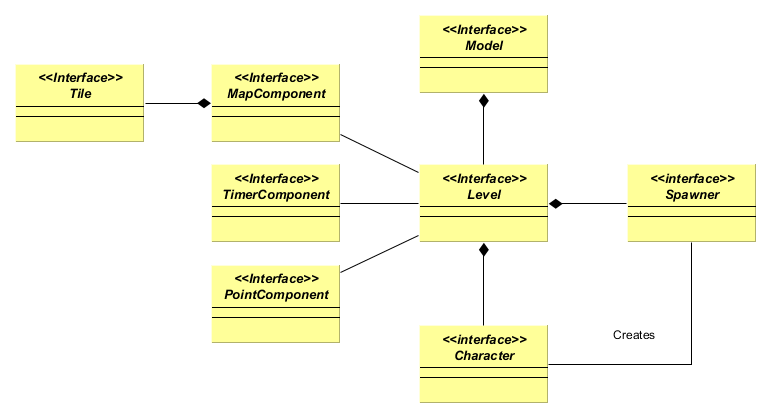
\includegraphics[width=\linewidth]{img/Analisi}
\caption{Schema dell'analisi e modello del dominio}
\label{img:Analysis}
\end{figure}

\chapter{Design}

\section{Architettura}

L'architettura dell'applicazione è realizzata utilizzando il pattern architetturale MVC in quanto permette facilmente di separare la logica e i dati della applicazione dalla effettiva tecnica adottata per la visualizzazione di questi. La applicazione e quindi la relativa architettura sono suddivise in varie implementazioni a seconda dello stato nelle quali si trovano.

L'interfaccia Model fornisce tutte le funzionalità comuni ad ogni stato della applicazione per comunicare al Controller i dati da mostrare e presentare i comandi capace di ricevere e in grado di influenzare l'esecuzione della logica interna. La gestione dello stato corrente e la relativa implementazione lato model è fatta da una entità preposta del Controller detta GameStatusManager.

\begin{figure}[H]
\centering{}
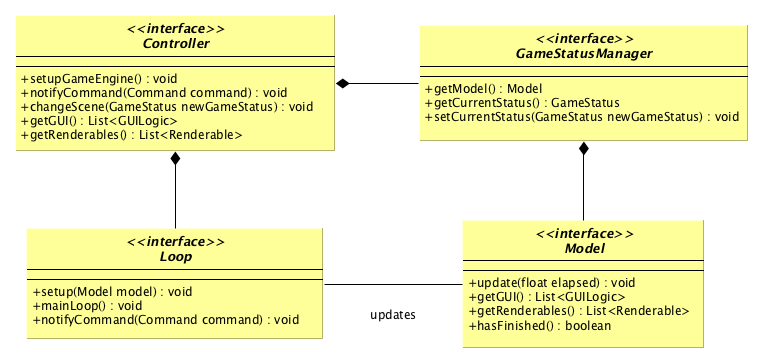
\includegraphics[width=\linewidth]{img/ArchitetturaControllerModel}
\caption{Il dialogo fra Controller e Model}
\label{img:ControllerModel}
\end{figure}

Il Controller si occupa principalmente di gestire il dialogo fra Model e View, oltre che di fornire numerose funzionalità per la lettura e scrittura su file di dfferenti tipi di dati persistenti. Il Controller deve inoltre gestire una componente vitale della applicazione detta Loop, che permette di aggiornare la grafica e la logica di gioco nel tempo, sostituendo il Model quando cambia lo stato del programma.

Il dialogo fra Controller e View è più stabile in quanto è la View stessa ad associare alle differenti scene lo stato di gioco e a realizzare effettivamente il cambio da una scena all'altra. \emph{Scene} svolge effettivamente la renderizzazione grafica sfruttando particolari classi, aggiornate dal Model, che confezionano tutti i dati necessari per disegnare correttamente immagini (\emph{Renderable}) e GUI (\emph{GUILogic}).

\begin{figure}[H]
\centering{}
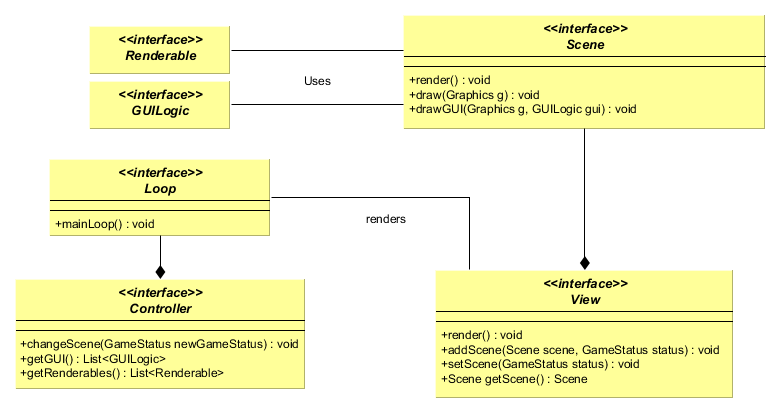
\includegraphics[width=\linewidth]{img/ArchitetturaControllerView}
\caption{Il dialogo fra Controller e View}
\label{img:ControllerView}
\end{figure}

\section{Design dettagliato}

\begin{flushright}
\item\subsubsection{Alessandro Lombardi - Logica dei personaggi}
\end{flushright}

I personaggi svolgono diverse azioni e fanno diverse scelte durante il loro ciclo di vita. Per evitare una gestione troppo cablata e poco mantenibile delle specifiche situazioni è stato scelto di utilizzare lo \textbf{State Pattern}. Il pattern State evita l'utilizzo di monolitici  blocchi condizionali all'interno delle classi dei singoli personaggi per la scelta e l’esecuzione di una azione piuttosto che un’altra, frammentando lo svolgimento delle singole azioni a classi specifiche che sono riutilizzabili e facilmente intercambiabili tra loro. Inoltre, permette di gestire meglio l'esecuzione delle animazioni e la simulazione delle attese che un personaggio fa fra un'azione e l'altra. Nella pratica ogni personaggio viene aggiornato col passare del tempo tramite il metodo update(float dt), ma questo delega completamente i propri compiti allo stato attuale.

Nel caso specifico  è stato scelto di associare a ciascun personaggio uno stato di riposo, reperibile tramite il metodo getStandingState() presente della interfaccia \emph{Character}, caratteristico per ciascuno e paragonabile a uno stato di attesa di una macchina a stati finiti responsabile delle maggiori scelte logiche del personaggio, come la strategia di movimento. La classe astratta \emph{CharacterStateImpl} è una semplice implementazione dell'interfaccia \emph{CharacterState} e viene ereditata direttamente dagli stati molto semplici o di transizione, come rispettivamente \emph{QbertStandingState} e \emph{LandState}. Le classi astratte \emph{WaitAnimationState} e \emph{WaitTimerState} invece, usano il metodo update() come \textbf{Template Method} per permettere alle classi concrete la personalizzazione nel metodo conclude() delle azioni da svolgere, rispettivamente alla fine di una animazione o allo scadere di un timer. \emph{MoveState} contiene gli stati usati da tutti i personaggi per eseguire i basilari movimenti nelle due o quattro direzioni a seconda del tipo di \emph{Character} che viene passato.

\begin{figure}[H]
\centering{}
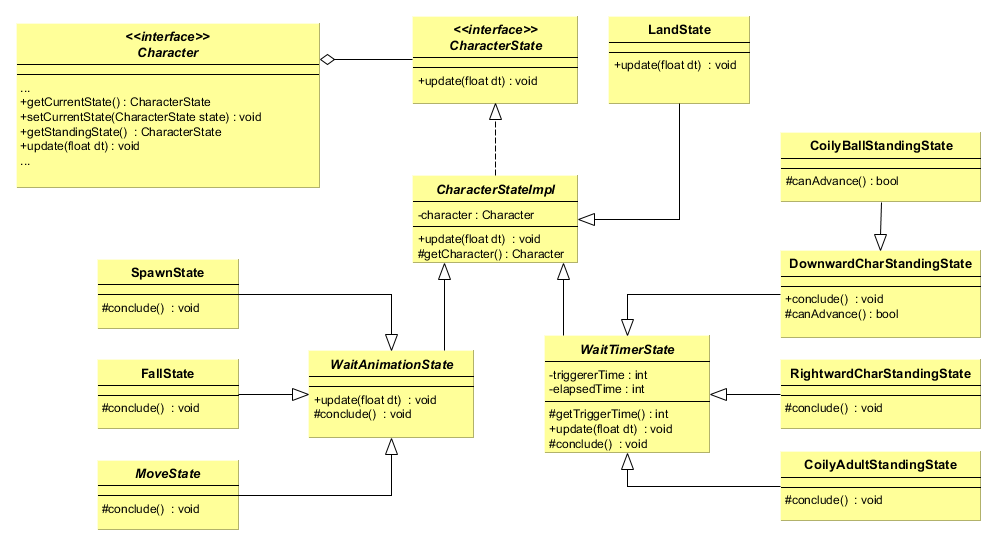
\includegraphics[width=\linewidth]{img/CharacterStates}
\caption{Alcune delle principali classi della gerarchia dei Character State}
\label{img:CharacterStates}
\end{figure}

E' importante sottolineare che gli stati vengono inizializzati passando il \emph{Character} associato, permettendo allo stato di applicarvi le modifiche necessarie, quindi i costruttori degli stati sono modellati per accettare anche le classi più specifiche della gerarchia dei personaggi, limitando e proteggendo gli stati che devono essere usati solo per certi personaggi. Ad esempio, \emph{QbertOnDiskState} accetta solo \emph{Player}, mentre \emph{FallState} può accettare un \emph{Character} oppure un \emph{DownUpwardCharacter} operando in modo differente.


\begin{figure}[H]
\centering{}
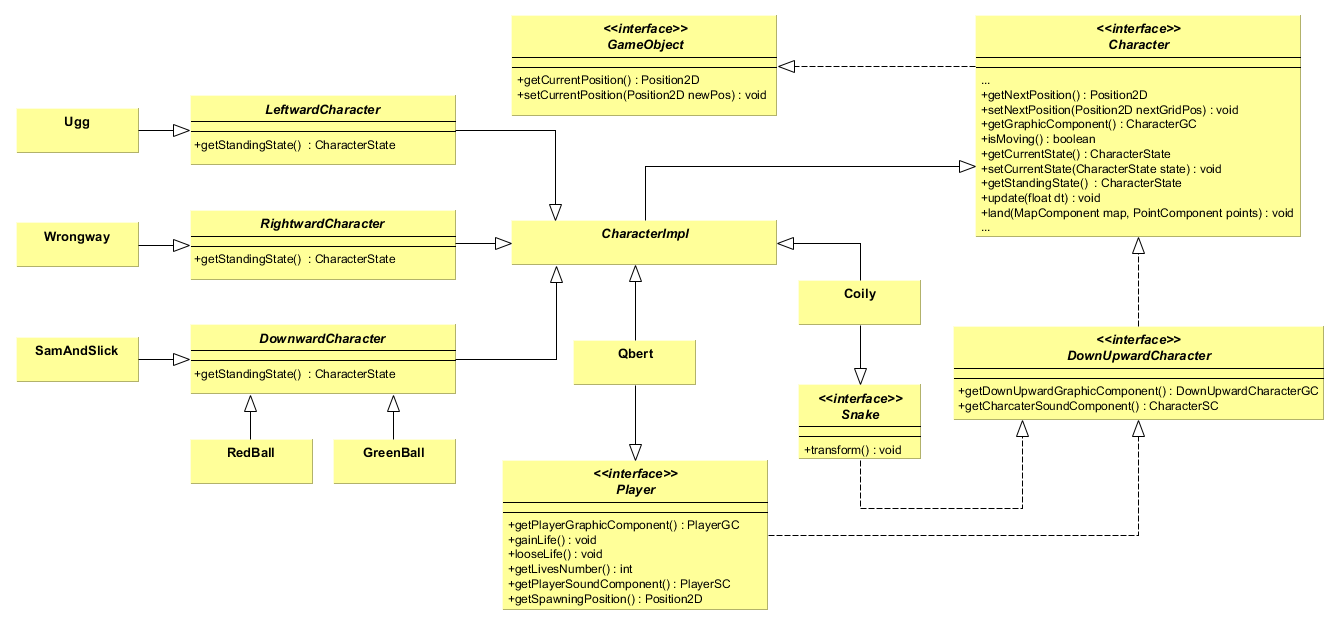
\includegraphics[width=\linewidth]{img/GerarchiaCharacters}
\caption{La gerarchia dei Character}
\label{img:GerarchiaCharacters}
\end{figure}

\begin{flushright}
\item\subsubsection{Alessandro Lombardi - Animazione dei personaggi}
\end{flushright}

Durante la fase di analisi è stato scelto di dividere quella che era la posizione "logica" del personaggio, ovvero la posizione nella griglia immaginaria disegnata dalle facce dei cubi del terreno di gioco, da quella "fisica", ovvero la coordinata del pixel nella finestra di gioco, dove si posiziona l'angolo in alto a sinistra dell'immagine rettangolare del personaggio. Questo ha comportato anche una divisione degli aspetti grafici da quelli logici e la scelta di considerare i movimenti come il salto, la caduta etc.. vere e proprie animazioni. La gestione dei dati necessari alla renderizzazione grafica dei personaggi, quali la posizione, lo sprite e la dimensione di questo, sono gestiti dalle classi che implementano \emph{CharacterGC}. Nella concezione del Graphic Component mi sono ispirato alla definizione di Component Pattern, un pattern molto comune nello sviluppo di videogiochi, sfruttando soprattutto la sua capacità di dividere le molteplici caratteristiche di natura diversa appartenenti allo stesso oggetto di gioco. Nel rispetto della architettura MVC, è importante precisare che i graphic component non svolgono nessuna operazione grafica. La gerarchia dei Character Graphic Component si basa sul riutilizzo del codice in comune e sulle animazioni supportate, \emph{CharacterGC} fornisce i metodi per la gestione delle animazioni e presenta quelle base. Le interfacce e le classi per la gestione della grafica di Coily e Qbert supportano animazioni per muoversi anche verso l'alto oltre che gestire gli sprite per il fronte e il dietro dei personaggi. Da notare come Coily sfrutti il metodo setFrontSprites(OneSideCharacterSprites frontSprites) per trasformarsi dalla palla viola che è inizialmente alla sua forma finale.

\begin{figure}[H]
\centering{}
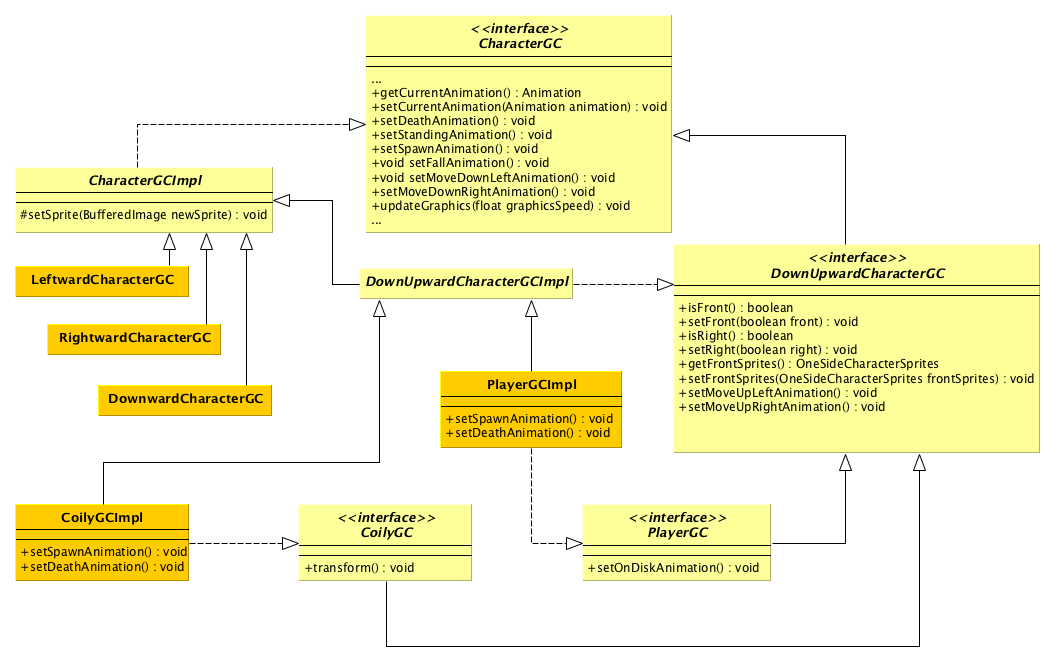
\includegraphics[width=\linewidth]{img/GerarchiaCGC}
\caption{La gerarchia CharcaterGC}
\label{img:GerarchiaCGC}
\end{figure}

Le animazioni dei personaggi sono state sviluppate sfruttando il pattern \textbf{Iterator} essendo queste delle sequenze di posizioni bidimensionali nella finestra di gioco. La interfaccia \emph{MovementAnimation} nasconde le modalità con le quali vengono fornite le posizioni e le condizioni di termine dell’animazione, per velocizzare lo scorrimento si può ricorrere a updateAnimation(int animationCycles) che permette di richiamare più volte il metodo next() e di ottenere il risultato finale. L’implementazione \emph{MovementAnimationImpl} di \emph{MovementAnimation} è una classe astratta che contiene l’implementazione dei metodi utili per gestire le posizioni ma che lascia alle classi concrete la politica di scorrimento, quindi il calcolo matematico delle posizioni, nel metodo next() invocato in updateAnimation(float animationSpeed) che fa quindi da \textbf{Template Method}. \emph{ComposedAnimation} permette di costruire animazioni più complesse, gestendo una coda di singole semplici animazioni e controllando l'esecuzione di queste.

\begin{figure}[H]
\centering{}
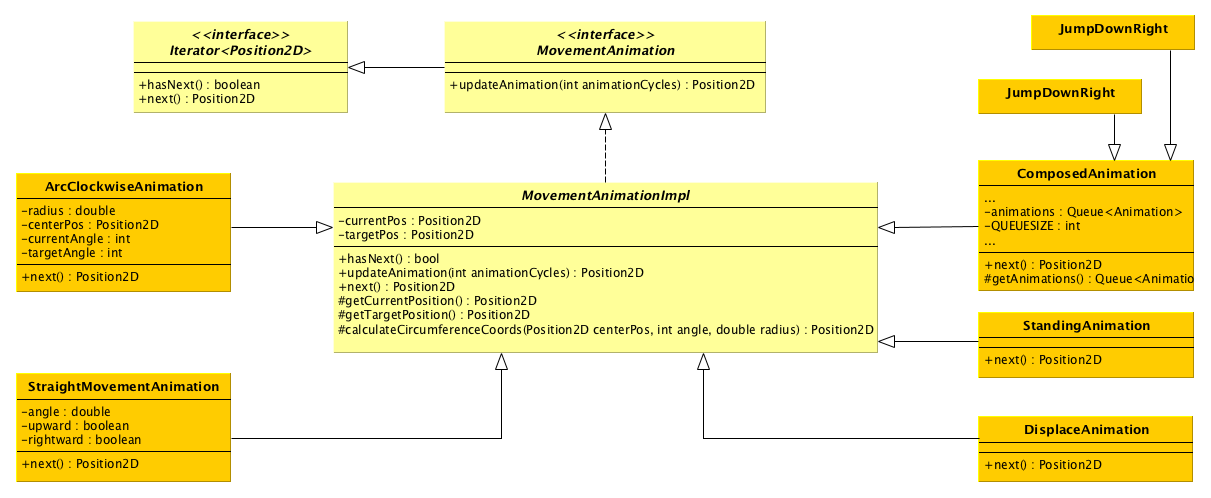
\includegraphics[width=\linewidth]{img/AnimazioniPersonaggi}
\caption{Alcune animazioni dei characters}
\label{img:AnimazioniPersonaggi}
\end{figure}

\begin{flushright}
\item\subsubsection{Marco Meluzzi - Lettura da file della configurazione dei livelli}
\end{flushright}

Per gestire le informazioni riguardanti la configurazione dei livelli e dei round dei quali si compone il gioco si è scelto di memorizzarle su file, per garantire una maggiore flessibilità delle stesse, anche nell'ottica di possibili cambiamenti. A tale scopo si è scelto di utilizzare un file .xml per l'espressività intrinseca al linguaggio di markup, reso ancor più semplice da gestire grazie all'impiego di un'apposita libreria, JDOM (illustrata nel dettaglio in \hyperlink{target}{seguito}). Per l'aumento graduale della difficoltà nell'avanzamento del gameplay si è scelto di replicare il più fedelmente possibile la configurazione di gioco dell'originale, almeno per quanto riguarda le tipologie di nemici da affrontare in ciascun round. In particolare, il metodo readLevelConfiguration(int levelNumber, int roundNumber), dopo aver ottenuto le informazioni necessarie al caricamento del round specifico, riempie una mappa costituita da elementi che hanno per chiave un personaggio (gestito tramite enumerazione) che il player deve affrontare e per valore una istanza della classe \emph{EnemyInfoImpl} contenente i valori di interesse per quel determinato soggetto che saranno validi per l'intera durata del round, vale a dire: la sua velocità, il numero di personaggi di quel tipo specifico che devono essere presenti "contemporaneamente" sulla mappa, la frequenza con la quale compaiono su di essa e il tempo di standing, necessario per gestire l'animazione. Questa mappa, insieme alle informazioni riguardanti più nello specifico l'ambiente di gioco, tra cui il numero di colori da impostare sui cubi, l'eventuale reversibilità degli stessi e il numero dei dischi, viene passata alla classe \emph{LevelSettingsImpl}, che conterrà quindi tutti i dati utili al caricamento del round corrente. Vengono altresì forniti alla classe sopra citata il colore dello sfondo e dei vari tile, elementi che andranno a costituire lo schema cromatico del round, scelto randomicamente tra configurazioni precedentemente stabilite dal singleton \emph{Sprites} e gestite attraverso \emph{ColorCompositionImpl}.

\begin{figure}[H]
\centering{}
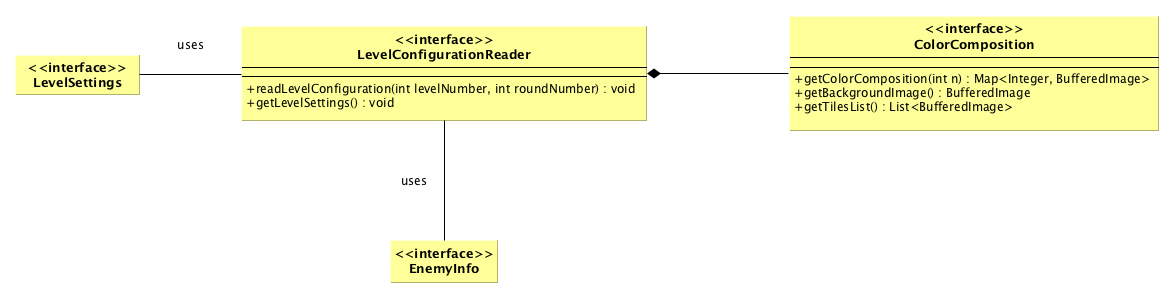
\includegraphics[width=\linewidth]{img/ComposizioneLivelli}
\caption{Lettura da file e composizione dei livelli}
\label{img:ComposizioneLivelli}
\end{figure}

\begin{flushright}
\item\subsubsection{Marco Meluzzi - Spawning}
\end{flushright}

La logica di spawning dei personaggi sulla mappa viene gestita dal metodo update(float dt) della classe \emph{SpawnerImpl}. Servendosi della mappa precedentemente realizzata da \emph{LevelConfigurationReaderImpl}, ad ogni ciclo del game loop viene controllato per ogni personaggio se il tempo trascorso dal suo ultimo spawning, ottenuto dal metodo getElapsedTime() di \emph{EnemyInfoImpl}, eccede la frequenza stessa di spawning, ottenuta da getSpawningTime(). In caso negativo si aggiorna il tempo trascorso attraverso incElapsedTime(float dt) e si passano in rassegna gli altri personaggi; altrimenti, viene resettato il timer associato a quel particolare personaggio e ne viene controllata la sua presenza sulla mappa. Solo se l'ammontare di quella particolare tipologia di personaggio correntemente sulla mappa (metodo getCurrentQuantity()) è inferiore al numero di sue presenze contemporanee permesse (metodo getTotalQuantity()) si procede con l'effettivo spawning. La composizione dei personaggi con le informazioni reperite da file avviene contestualmente, servendosi del pattern \textbf{Factory Method}, in modo da incapsulare le istanziazioni delle classi concrete. I personaggi così istanziati vengono aggiunti ad una lista di \emph{Character}, che esternamente verrà utilizzata e via via aggiornata da \emph{UpdateManager}, che si occupa altresì di richiamare il metodo death(Character character) di \emph{SpawnerImpl} che aggiorna (decrementandolo) il computo delle istanze della tipologia di personaggio in questione attualmente sulla mappa.

\begin{figure}[H]
\centering{}
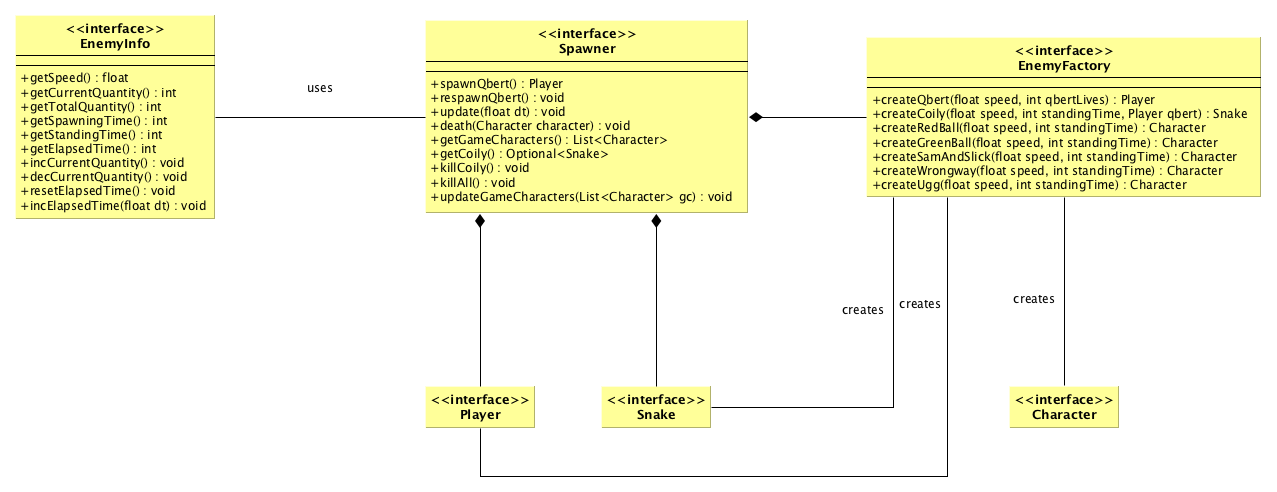
\includegraphics[width=\linewidth]{img/CreazioneNemiciESpawner}
\caption{Creazione dei nemici e loro spawning}
\label{img:CreazioneNemiciESpawner}
\end{figure}

\begin{flushright}
\item\subsubsection{Marco Meluzzi - Effetti sonori}
\end{flushright}

Per l'implementazione degli effetti sonori si è cercato di procedere in maniera analoga alla gerarchia realizzata per la gestione dei dati necessari alla renderizzazione grafica dei personaggi. Si è quindi sviluppata l'interfaccia base \emph{SoundComponent} che esplicita i metodi comuni a tutte le sottointerfacce e che rappresenta l'interfaccia necessaria alle classi concrete che gestiscono i suoni legati all'avvio del gioco e ai round. Scendendo nella gerarchia vi sono poi le interfacce \emph{CharacterSC}, riguardante i personaggi che si muovono sulla mappa, e \emph{PlayerSC} che gestisce i suoni legati a Qbert. Le classi che lo richiedono si compongono quindi di un oggetto Sound Component responsabile della gestione dei suoni ad esse associati, mentre, quando ciò è possibile, la gestione dei suoni è associata direttamente agli stati legati ai personaggi. Ogni volta che nel model si verifica un evento a cui deve corrispondere la riproduzione di un effetto sonoro, viene creata la Clip corrispondente mediante il metodo uploadClip(SoundEffectFile soundEffect) di \emph{ControllerImpl} che carica il suono da file e lo inserisce in una coda. A questo punto, chiamando il metodo notifyPlaySound() e passando attraverso il metodo emptyClipQueue(Queue$\langle Clip \rangle$ queue) di \emph{ControllerImpl}, viene invocato il metodo play(Queue$\langle Clip \rangle$ clipToPlay) in \emph{ViewImpl} che riproduce effettivamente il suono rimuovendolo dalla coda.

\begin{figure}[H]
\centering{}
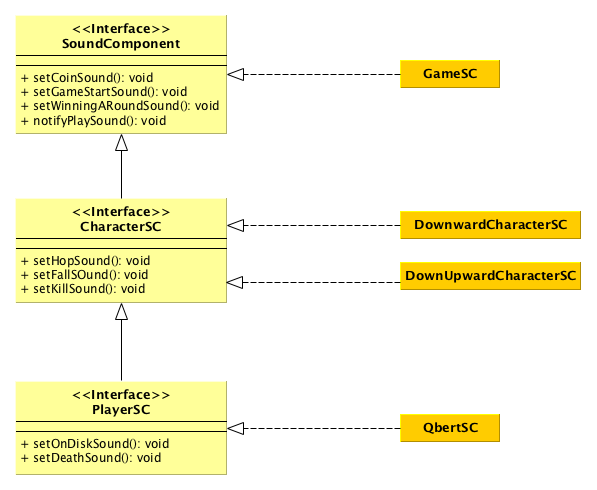
\includegraphics[width=\linewidth]{img/GerarchiaSound}
\caption{La gerarchia per la gestione degli effetti sonori}
\label{img:GerarchiaSound}
\end{figure}

\begin{flushright}
\item\subsubsection{Alessandro Stockman - Sviluppo di Level}
\end{flushright}

La classe \emph{Level} è stata pensata con un ruolo principale nella gestione delle meccaniche di gioco. Per evitare la creazione di una classe monolitica contente aspetti completamente diversificati tra loro è stato scelto di sviluppare un insieme di classi \emph{Component}.
In particolare vengono sviluppati un \emph{MapComponent} per la gestione di aspetti riguardanti il mondo di gioco (tile, dischi, controllo cadute, ...).
Un \emph{PointComponent} per la gestione dei punti e delle vite guadagnate con essi, contenente i valori costanti dei punteggi ottenuti al verificarsi di dati avvenimenti.
Un \emph{TimerComponent}, gestore dei vari update alle entità di gioco, approfondito più avanti.

\begin{figure}[H]
\centering{}
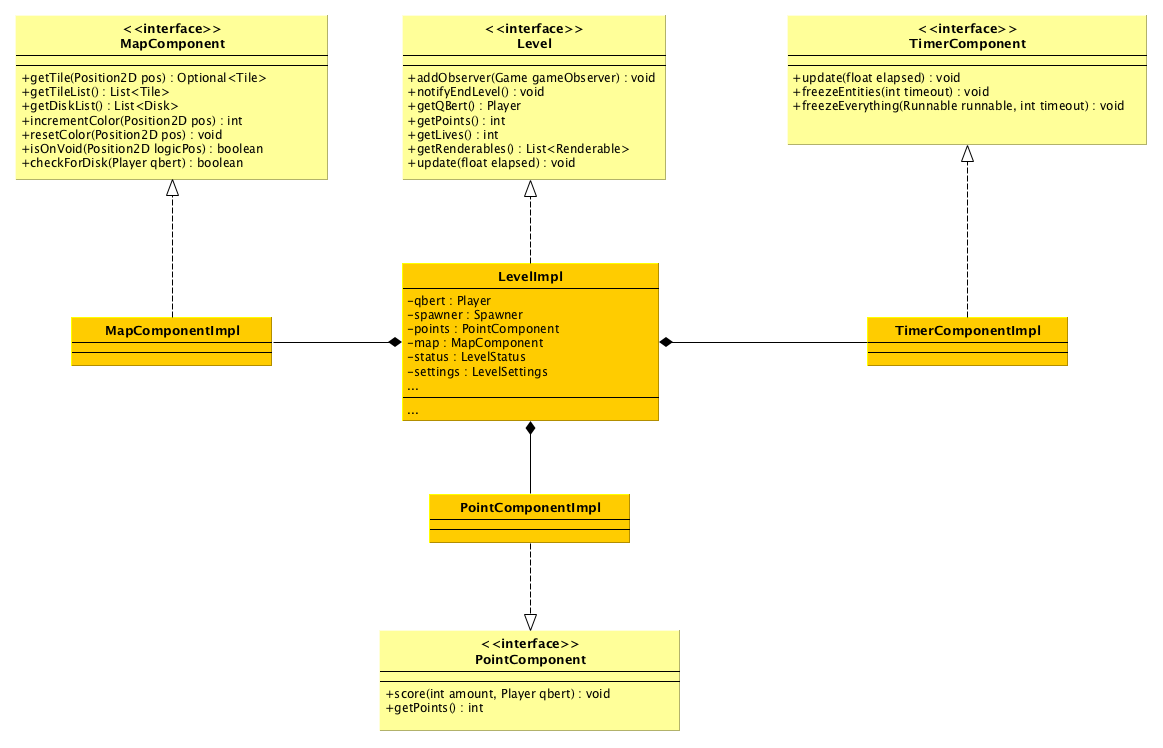
\includegraphics[width=\linewidth]{img/LevelArchitecture}
\caption{Gerarchia dei Component di Level}
\label{img:LevelArchitecture}
\end{figure}

\begin{flushright}
\item\subsubsection{Alessandro Stockman - Gestione delle Collisioni}
\end{flushright}

Data la necessità di realizzare un set di personaggi con caratteristiche differenti tra di loro e più in particolare con diversi tipi di reazioni comportamentali alla collisione con il giocatore si è scelto di utilizzare il \textbf{Template Method} checkCollision() nella classe astratta \emph{CharacterImpl} per permettere ad ogni personaggio di implementare un'azione personalizzata all'esecuzione di collide() sfruttando i vari \emph{Component} che gli vengono passati.
In questa maniera si introduce la possibilità di rendere più semplice l'introduzione di personaggi nel gioco con nuovi effetti che possono manipolare il flusso del gioco.

\begin{figure}[H]
\centering{}
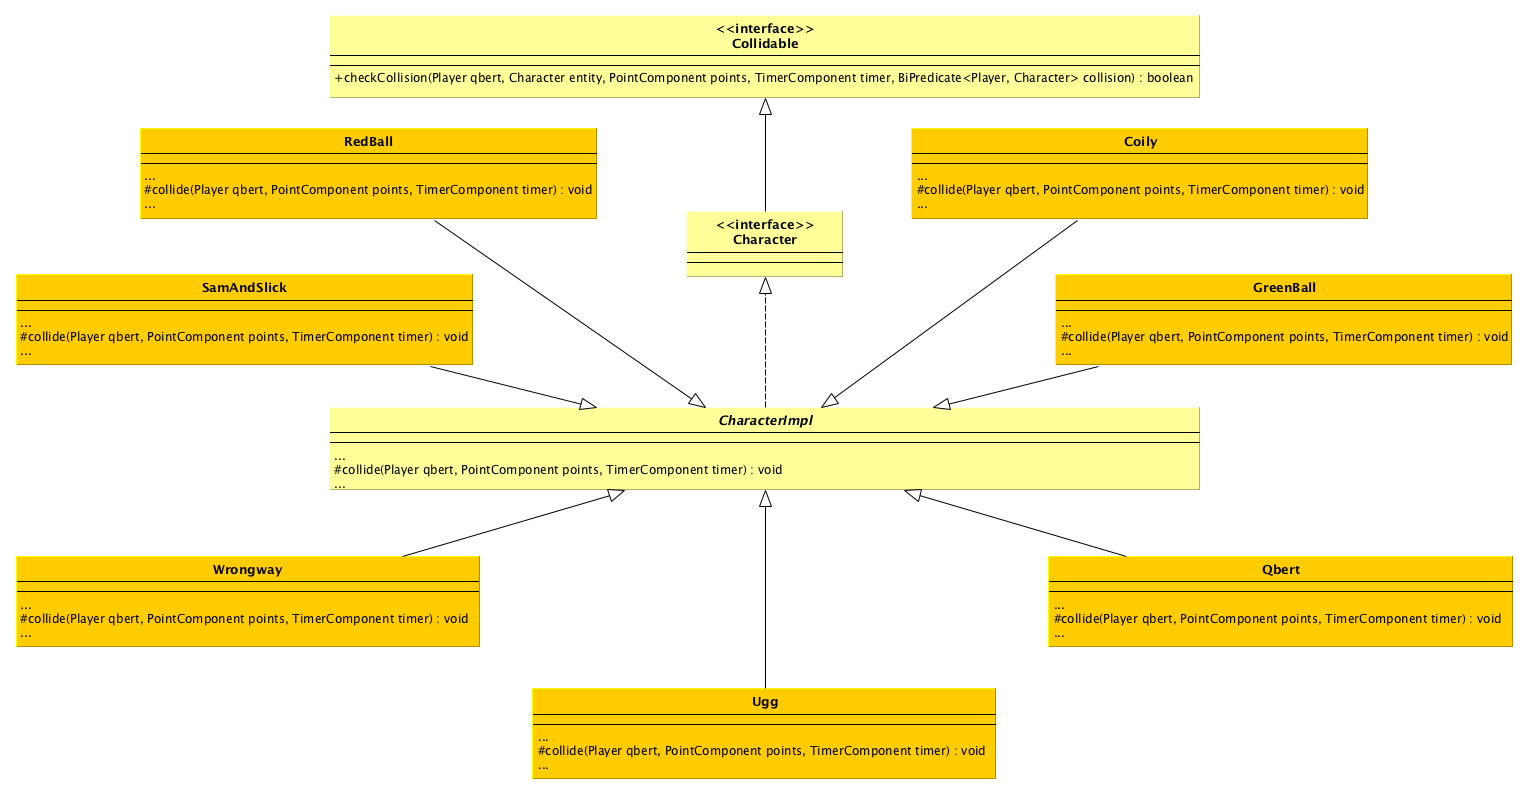
\includegraphics[width=\linewidth]{img/CheckCollision}
\caption{Schema dettagliato della gestione comportamentale delle collisioni}
\label{img:CheckCollision}
\end{figure}

Durante la fasi di analisi si è optato per un controllo delle collisioni a livello puramente logico, senza quindi controllare le posizioni fisiche degli sprite nella finestra ma solo la loro posizione in coordinate all'interno della mappa. Nonostante l'appartente comodità di questo tipo di gestione in contesto simile si è presentata la necessità di dover verificare più volte la presenza di collisioni nel corso di un solo ciclo di update. Per semplificare il processo si è deciso di utilizzare il pattern \textbf{Strategy}, realizzato con l'implementazione dell'interfaccia funzionale \emph{BiPredicate$\langle X, Y \rangle$} utilizzata come \emph{BiPredicate$\langle Player, Character \rangle$}. La classe implementativa della strategia viene istanziata e passata come parametro al metodo checkCollision(), che facendo un test sull'istanza può determinare se ci sia una collisione in atto.

\begin{figure}[H]
\centering{}
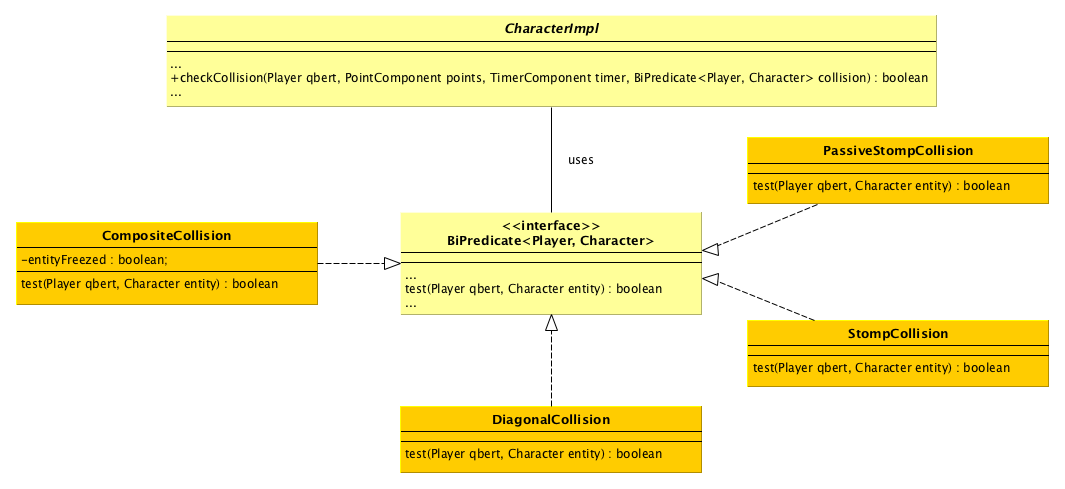
\includegraphics[width=\linewidth]{img/CollisionStrategy}
\caption{Implementazione del Pattern Strategy per la gestione delle collisioni}
\label{img:CollisionStrategy}
\end{figure}

\begin{flushright}
\item\subsubsection{Alessandro Stockman - Flusso temporale del gioco}
\end{flushright}

Per gestire in maniera comoda le alterazioni del flusso temporale durante il gioco (freeze dei nemici in seguito alla cattura di \emph{GreenBall}, attesa di pochi secondi dopo una morte o vincita del livello, ...) si è optato per la realizzazione del pattern \textbf{Strategy} al fine di dare la possibilità al metodo update() di \emph{TimerComponent} di implementare diversi algoritmi a seconda delle necessità.
Questa gestione permette inoltre di poter introdurre ottimalmente nuovi algoritmi di update senza alterare enormemente il codice.

\begin{figure}[H]
\centering{}
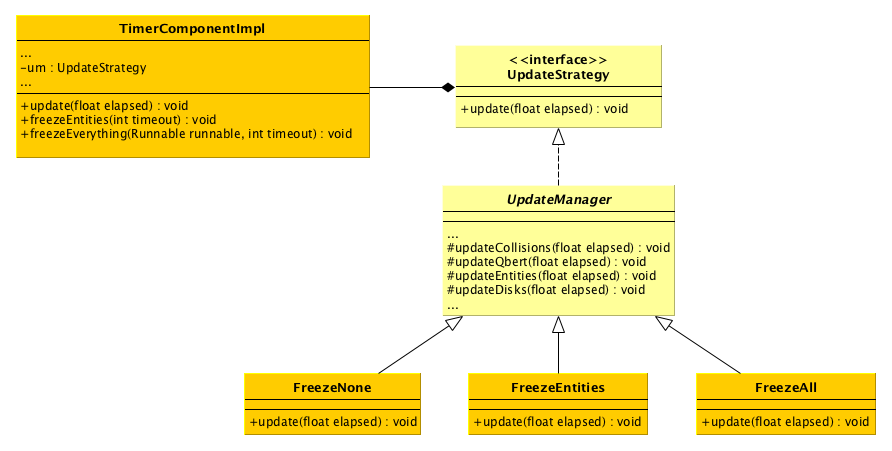
\includegraphics[width=\linewidth]{img/UpdateStrategy}
\caption{Implementazione dei vari algoritmi di Update}
\label{img:UpdateStrategy}
\end{figure}

\begin{flushright}
\item\subsubsection{Andrea Giulianini - Gestione Risoluzione/Immagini}
\end{flushright}

Per far si che l'interfaccia fosse il più responsive possibile avevamo bisogno di alcune informazioni, ci serviva sapere quanti pixel componevano il display su cui sarebbe dovuta girare l'applicazione.

Avendo creato le immagini che compongono il gioco in un formato vettoriale (SVG) potevamo tramite l'utilizzo di varie librerie (\emph{Batik} con tutte le sue dipendenze) creare immagini raster di dimensioni e pesantezza adeguate all'interfaccia su cui sarebbe girata l'applicazione. Quindi vengono caricati tutti i nomi dei file da convertire un file \emph{imageconfig.txt}, creando quindi una classe specifica \emph{LoadResources} vado ad effetture al lancio dell' applicazione la conversione delle immagini, posizionando l'output ottenuto raster in una cartella specifica nella directory \emph{home/qbert} dell'utente.

\begin{flushright}
\item\subsubsection{Andrea Giulianini - Gestione degli Input}
\end{flushright}

Per gestire gli input dell'utente, siccome questi sarebbero cambiati per ogni sezione del gioco, si è deciso di applicare il \textbf{Pattern Command}. Creo così l'interfaccia e le varie classi che andranno poi a gestire ogni singolo input possibile da tastiera. L'input viene chiamato dalla \emph{Scene}, la gestione poi del comando poi passerà al \emph{Controller} e succesivamente al \emph{GameEngine} che notificherà l'arrivo del comando al rispettivo model della scena, tutti questi passaggi avvengono tramite il notifyCommand(), il model gestirà il comando.

\begin{figure}[H]
\centering{}
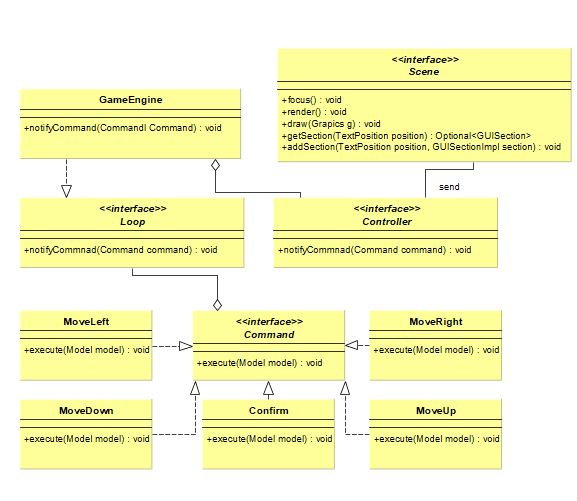
\includegraphics[width=\linewidth]{img/PatternCommand}
\caption{La gerarchia per la gestione degli input}
\label{img:GerarchiaSound}
\end{figure}

\begin{flushright}
\item\subsubsection{Andrea Giulianini - Gestione del Ranking}
\end{flushright}

Si voleva gestire l'inserimento del nome a fine partita dell'utente, quindi ho deciso di creare una classe per la gestione dei dati che dovranno poi andare scritti sul file nel quale vengono memorizzati quest'ultimi. Siccome l'aggiunta del nome utente avviene tramite l'inserimento di sigoli caratteri selezionandoli a schermo, ho optato per una costruzione usando il \textbf{Pattern Builder}.
Quindi il model appena riceve dal \textbf{Pattern Command} l'input vede se deve aggiungere una lettera al nome.
In caso positivo esegue addChar, appena il nome è completo, quindi arriva l'input di conferma si builda l'oggetto, passando il return del metodo toString() al controller si andrà a scrivere su file \emph{ranking.txt} il punteggio più i relativi dati

\begin{figure}[H]
\centering{}
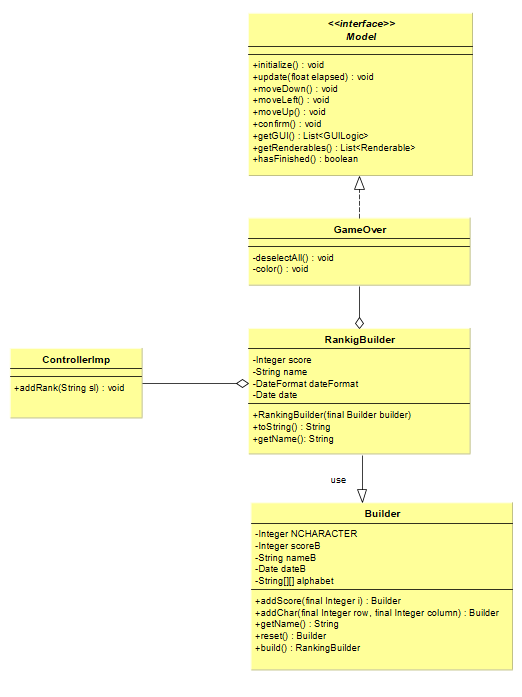
\includegraphics[width=\linewidth]{img/PatternBuilder}
\caption{La gerarchia per la gestione del ranking}
\label{img:PatternBuilder}
\end{figure}


\chapter{Sviluppo}
\section{Testing automatizzato}

Nelle classi di testing sono stati testati gli stati dei personaggi, per controllare anche la corretta esecuzione delle animazioni e delle transizioni indipendenti e il builder per aggiungere nuovi punteggi e la lettura da file di questi.

E' necessario predisporre delle cartelle con le immagini prima di eseguire i test, quindi giocare lanciare almeno una volta l'applicativo

Sono stati eseguiti anche dei test manuali sui sistemi operativi Windows, macOS e Linux, riscontrando il corretto funzionamento della applicazione, fatta eccezione per il suono che su Linux smette di funzionare dopo un po'. Inizialmente il problema si presentava anche eseguendo il JAR su Windows, ma a seguito di alcune modifiche sulla lettura delle risorse è stato risolto, mentre per Linux anche dopo una lunga ricerca non siamo riusciti a risolverlo. Provando l'applicazione in risoluzioni differenti può accadere che su alcune, le facce superiori dei cubi della mappa vengano sfasate, questo è causato dal fatto che le dimensioni delle immagini e le coordinate dei pixel sullo schermo essendo numeri interi non hanno la stessa precisione dei calcoli fatti per posizionarle.

\section{Metodologia di lavoro}

La suddivisione del lavoro è stata concepita con lo scopo di lasciare molta indipendenza fra i componenti del gruppo, nel rispetto dei tempi e degli impegni di ciascuno. Dopo una prima fase di analisi utile soprattutto a definire il dominio e confermare la suddivisione del lavoro, si è cercato di produrre un prototipo funzionante che permettesse la gestione dei movimenti e delle collisioni dei primi personaggi. La scelta e la implementazione del loop di gioco è stata fatta assieme, mentre ciascuno ha poi proseguito indipendentemente nel proprio lavoro, non mancando mai a comunicare, chiedere anche solo consigli al resto del gruppo. La parte di Model è stata predominante durante questa fase di sviluppo, concentrando il gruppo principalmente nella realizzazione sempre più dettagliata del gioco, includendo pian piano tutte le regole, i personaggi fondamentali e la gestione del punteggio. Con il Model pressochè ultimato e la necessità di aggiungere altre funzionalità alla applicazione si è ampliato la parte di Controller relegato al controllo del game loop alla gestione di più schermate con l'introduzione di scene e parti di View fino a quel momento ignorate nella implementazione. In generale lo sviluppo è stato un processo a spirale dovuto non solo alle correzioni e i miglioramenti architetturali e di dettaglio del codice ma anche alle tempistiche diverse dei membri del gruppo che seppur autonomi si sono mantenuti paralleli.
Nello specifico la divisione dei compiti è stata la seguente:
\begin{itemize}
	\item \textbf{Giulianini Andrea}: Gestione della dimensione dell'interfacia, con relativa conversione delle immagini a seconda della risoluzione del display, creazione delle varie scene estranee a quelle predisposte per il gioco, leggere e scrivere da file, per gestione ranking e lettura immagini

	\item \textbf{Lombardi Alessandro}: Realizzazione dei personaggi, sia negli aspetti grafici, animazioni e sprites, che in quelli logici, comportamento e strategia di movimento. Gestione dialogo model-view per la gestione della GUI, incapsulamento delle informazioni lato model, come testo e selezione, stilizzazione e formattazione lato view a seconda della parte di pagina occupata. Disegno delle risorse grafiche in formato vettoriale.

	\item \textbf{Meluzzi Marco}: Configurazione dei livelli e dei round di gioco, specificando le tipologie e il numero di personaggi presenti in ciascun round, la loro frequenza di spawning sulla mappa e la loro velocità, così come il numero di colori da impostare sui cubi e la loro eventuale reversibilità. Lettura di queste informazioni da file. Composizione dei round e dei personaggi con le informazioni acquisite e gestione dello spawning vero e proprio sulla mappa di gioco. Gestione degli effetti sonori.

	\item \textbf{Stockman Alessandro}: Creazione e gestione della mappa di gioco e dei controlli relativi a cadute ed utilizzo di Dischi. Logiche di funzionamento dei Tile e dell'interazione dei personaggi di gioco su di essi, gestione della colorazione di Tile standard e con colori a rotazione. Sistema di punteggio. Gestione del flusso di update dei vari attori del gioco. Controllo del superamento del round. Gestione delle collisioni.

\end{itemize}

\section{Note di sviluppo}

	\item \textbf{Giulianini Andrea}: Per la conversione delle immagini ho fatto affidamento ad una libreria molto documentata ed usata \href{https://xmlgraphics.apache.org/batik/using/swing.html}{Batik}, aumentando così la qualità degli sprites, avendo sempre delle dimensioni perfette per l'utilizzo.

	\item \textbf{Lombardi Alessandro}: Nello sviluppo delle animazioni e poi successivamente della GUI ho approfondito alcuni aspetti non trattati a lezione circa il funzionamento con il quale swing e awt effettuano il "painting" e la possibile personalizzazione di questo per la nostra applicazione. Sempre nella gestione della GUI ho fatto uso della classe Optional per controllare la presenza o meno nelle varie scene delle implementazioni lato view delle parti di una finestra (\emph{Optional$\langle GUISection \rangle$}) e del font. Per il posizionamento centrale delle stringhe basato sulla grandezza della finestra e del font mi sono rivolto a chi lo aveva fatto prima di me (\href{https://stackoverflow.com/questions/27706197/how-can-i-center-graphics-drawstring-in-java}{link}). Ho sfruttato l'API fornita da Java per la gestione di un minimale sistema di logging su file XML o su console, per scopi di debug ma anche segnalazione di errori  fatali per la applicazione.

	\hypertarget{target}{\item \textbf{Meluzzi Marco}}: Per la realizzazione della configurazione dei vari round di gioco, ho deciso di memorizzare le informazioni di interesse in un file .xml, per sfruttare i vantaggi derivanti dall'utilizzo del linguaggio di markup. A tal fine ho sfruttato ed approfondito personalmente la libreria \href{http://www.jdom.org}{JDOM 2.0.6}, che permette un accesso e una gestione molto semplice del file. Nello specifico, questo viene trattato secondo una visione gerarchica ad albero per cui, dopo aver istanziato il builder e con il metodo build(String arg0) aver ottenuto il Document che rappresenta il file, lo si può scorrere partendo dal suo elemento nella radice, ottenibile con il metodo getRootElement(), per passare poi ai livelli sottostanti mediante l'uso iterato di getChild(). Giunti ad un qualsiasi livello di profondità, il metodo getAttributeValue(String attname) permette di ottenere il valore corrispondente al parametro passato come argomento. Nel caso specifico in esame, una volta lette le informazioni inerenti a un dato round, ho proceduto a ricavare la lista dei nodi figli - rappresentanti i personaggi del round - con la chiamata a getChildren() e a crearne un iteratore, in modo da ciclare i nodi con gli usuali metodi dell'interfaccia \emph{Iterator} e ottenerne i parametri corrispondenti.

	\item \textbf{Stockman Alessandro}: Ho fatto largo utilizzo di stream nell'interezza dell'applicazione, ad esempio nella gestione del controllo delle collisioni, dove ho utilizzato anche lambda expressions al loro interno, o nel raggruppamento dei vari elementi di gioco renderizzabili in un unica lista nel metodo getRenderables() della classe \emph{LevelImpl} che vengono successivamente disegnati sulla view ordinati per l'indice restituito dal metodo getZIndex() dell'interfaccia \emph{Renderable} utilizzando una lambda expression.
	Inoltre dove necessario, come per esempio nella gestione del nemico Coily o in quella dei Dischi sulla mappa, ho utilizzato Optional non potendo garantire a priori la presenza delle istanze.
	Nella necessità di realizzare un timer con callback al suo termine ho utilizzato un piccolo snippet di codice trovato sul web (\href{https://stackoverflow.com/questions/26311470/what-is-the-equivalent-of-javascript-settimeout-in-java}{link}) che propone lo stesso comportamento della funzione setTimeout() di JavaScript.

\chapter{Commenti finali}


\section{Autovalutazione e lavori futuri}

	\item \textbf{Giulianini Andrea}: All'interno del gruppo probabilmente ero il meno convinto dal progetto, non per la sua complessità tanto quanto per l'idea del gioco, che non mi ha mai appassionato.
	
Tolto questo ho sempre cercato di comunicare con il gruppo cercando di capire quali fossero le necessità durante lo sviluppo, in modo tale da poter dare il giusto supporto al team. Ritengo comunque che la mia più grave mancanza sia stata quella di non aver operato in punti nevralgici del gioco, concentrandomi solo su aspetti "secondari".

Mi sono concentrato su lettura e scrittura su file e su tutte quelle interfaccie non prettamente inerenti al gioco, per esempio gestendo il ranking o la grandezza delle immagini.

Non credo che lavorerò più sul progetto, non avendomi conquistato, ma credo comunque che l'epserienza maturata mi abbia aiutato a riflettere di più sulla fase di progettazione e della sua importanza.

	\item \textbf{Lombardi Alessandro}: Mi posso reputare complessivamente soddisfatto del lavoro da svolto durante tutte le fasi del progetto, oltre che divertente, è stata una esperienza tutto sommato costruttiva. La scelta di un videogioco credo abbia permesso la creazione di un mondo virtuale pieno di dettagli, la maggior parte da costruire e progettare partendo da zero, stimolando l'ingegno e l'interesse nel creare il meglio possibile complesse gerarchie. Nella creazione dei personaggi penso di aver svolto principalmente un esercizio avanzato sulle fondamenta della programmazione ad oggetti, cercando il più possibile di riutilizzare il codice e di strutturarlo il meglio possibile. Nella realizzazione degli aspetti grafici invece mi sono interessato ad argomenti più particolari o ho fatto la conoscenza di alcuni totalmente nuovi. In entrambi i casi ho colto l'occasione per leggere materiale riguardante i pattern di programmazione e conoscere nuovi argomenti. Sia per le motivazioni precedentemente dette che probabilmente per una divisione del lavoro inconsapevolmente poco equilibrata sul lato qualitativo, ovvero divisa in parti con contenuti completamente differenti una dall'altra, penso che una grande mancanza nella mia parte sia stata quella di non aver usato alcuna libreria. Personalmente ho mantenuto sempre un dialogo, quasi costante, con i singoli membri del gruppo, trovandomi spesso a fare da ponte nella comunicazione degli aggiornamenti o tenere traccia della realizzazione del progetto, è anche questa una parte dell'esperienza formativa del progetto. Sono soddisfatto che il gruppo sia sempre stato disponibile ad aiutarmi e farsi aiutare. Non credo che lavorerò ulteriormente a questo progetto, anche se può darsi che in futuro lo riprenda come spunto.

	\item \textbf{Meluzzi Marco}: Reputo l'esperienza di realizzazione di questo progetto senz'altro formativa, più per l'avere imparato come si deve procedere quando si lavora in un team che per l'aver appreso metodologie vincenti di progettazione, cosa che, personalmente, sento l'esigenza di dover apprendere da una figura esterna, almeno per acquisire le basi necessarie che consentano poi di crescere e migliorarsi autonomamente. Essendo infatti questo un progetto di discreta complessità, è stato per me, soprattutto nella fase iniziale, abbastanza faticoso gestire l'architettura generale e approcciarmi ad essa, specialmente quando era necessario entrare nell'ottica di quanto già prodotto dagli altri, nel momento in cui le parti realizzate singolarmente dovevano interfacciarsi e comunicare direttamente. Ho fatto presente al gruppo questa mia necessità alla quale i miei compagni hanno sempre cercato di porre rimedio aiutandomi nella comprensione generale e poter quindi procedere. D'altro canto, aver dovuto affrontare queste difficoltà è servito a rendere nel complesso il codice il più possibile coerente nelle sue parti, sfruttando laddove possibile tecniche di progettazione già utilizzate all'interno del progetto e rivelatesi convenienti.
	
Nonostante inizialmente fossi dubbioso circa la praticità nell'utilizzare il DVCS, man mano che acquisivo confidenza con lo strumento ne ho apprezzato sempre più le potenzialità che lo rendono di fatto un elemento difficilmente sostituibile in un contesto di lavoro di gruppo come questo, permettendo alle varie parti di coordinarsi efficientemente, malgrado le incertezze iniziali forse dovute alla poca dimestichezza con i comandi. 

Conoscendo le mie capacità e i miei limiti, mi ritengo relativamente soddisfatto di quanto prodotto, con la consapevolezza di non aver messo in piedi un'architettura solida come auspicavo, ma comunque gratificato dall'essere riuscito a portare a termine un progetto di queste dimensioni, finora mai affrontato. Non penso che porterò avanti questo progetto, ma certamente ha contribuito in modo non indifferente a farmi capire la direzione giusta da prendere per affrontare lavori simili in futuro.

	\item \textbf{Stockman Alessandro}: Nel complesso ho trovato lo sviluppo del progetto particolarmente impegnativo e molto probabilmente a causa dell'averlo sottovalutato nelle fasi iniziali, in cui, oltre alla difficoltà del realizzare un progetto di modeste dimensioni in un gruppo di quattro elementi, esisteva la necessità di formare delle basi per quanto riguarda l'ambito dello sviluppo dei videogiochi e applicare Design Pattern e architettura MVC in un contesto decisamente più impegnativo del solito.
	
In ogni caso mi reputo relativamente soddisfatto dei risultati del mio lavoro, nonostante molto al di sotto delle mi aspettative iniziali, soprattutto per quanto riguarda la quantità di Pattern implementati. Il lavoro svolto è comunque sicuramente riuscito a dare molta più profondità alle mie conoscenze.

\section{Difficoltà incontrate e commenti per i docenti}

La difficoltà principale nella realizzazione del progetto è stata quella di eleborare l'architettura della applicazione, in quanto mancava una esperienza pratica sull'argomento e per alcuni membri del gruppo la costruzione di una applicazione completa, usando un linguaggio orientato agli oggetti, era una esperienza totalmente nuova. Rispetto ad altri argomenti trattati molto approfonditamente, e quindi sotto il nostro pieno controllo, l'architettura ci ha posto troppi interrogativi e molto timore nelle scelte fatte.

\appendix
\chapter{Guida utente}

\section{Il gioco}

\subsubsection{Scopo del gioco}

Il giocatore ha come obiettivo quello di colorare tutti i cubi della mappa di un certo colore che di volta in volta viene indicato in alto a sinistra nella schermata di gioco e accumulare in questo modo più punti possibili. Procedendo con i livelli, i cubi potrebbero diventare reversibili, vale a dire che una volta raggiunto il giusto colore, un ulteriore salto sulla sua superficie lo farebbe tornare al colore di partenza. Ad ostacolare o, in alcuni casi, aiutare il giocatore c'è una schiera di diversi personaggi, che si muovono e si comportano in maniera differente sulla mappa:

\subsubsection{I personaggi}

\begin{figure}[H]
		\item
		
\includegraphics[width=0.15\linewidth]{img/Qbert}
		\label{img:Q*Bert}
		\textbf{Q*Bert}

		Protagonista che il giocatore deve comandare: può cambiare il colore dei cubi saltando in quattro direzioni diverse: in alto a destra, in alto a sinistra, in basso a destra e in basso a sinistra. Possiede un numero limitato di vite, che può incrementare raggiunta una certa soglia di punteggio. Cadere oltre i bordi della mappa, o entrare in contatto con uno dei suoi nemici, gli fa perdere una vita.

\end{figure}

\begin{figure}[H]
		\item
		
\includegraphics[width=0.15\linewidth]{img/PurpleBall}
		
\includegraphics[width=0.15\linewidth]{img/Coily}
		\label{img:Coily}
		\textbf{Coily}

		Principale antagonista di Q*Bert. All'inizio del round appare in cima con le sembianze di una palla viola che scende lungo la mappa: raggiunto il fondo si trasforma in un serpente che insegue Q*Bert nei suoi spostamenti. L'unico modo per eliminarlo è far saltare Q*Bert su un disco quando si trova vicino a lui: in questo modo Coily proverà a seguirlo e nel tentativo cadrà dalla mappa... finché non apparirà nuovamente in cima alla piramide sotto forma di palla viola.

\end{figure}

\begin{figure}[H]
		\item
		
\includegraphics[width=0.15\linewidth]{img/RedBall}
		\label{img:RedBall}
		\textbf{RedBall}

		Le palle rosse sono un ostacolo per Q*Bert. Queste appaiono in cima alla mappa e proseguono rimbalzando verso il basso seguendo un percorso randomico, cadendo una volta raggiunto il fondo della mappa. Ogni contatto con Q*Bert causerà a quest'ultimo la perdita di una vita.

\end{figure}

\begin{figure}[H]
		\item
		
\includegraphics[width=0.15\linewidth]{img/GreenBall}
		\label{img:GreenBall}
		\textbf{GreenBall}

		Le palle verdi assumono lo stesso comportamento delle palle rosse, ma sono un aiuto per Q*Bert: toccandole, infatti, il tempo di gioco viene fermato per qualche secondo, permettendo a Q*Bert di saltare per la mappa in relativa sicurezza.

\end{figure}

\begin{figure}[H]
		\item
		
\includegraphics[width=0.15\linewidth]{img/Wrongway}
		
\includegraphics[width=0.15\linewidth]{img/Ugg}
		\label{img:Wrongway&Ugg}
		\textbf{Wrongway e Ugg}

		Questi due personaggi ostacolano Q*Bert, ma si comportano in maniera differente rispetto agli altri. Wrongway appare nell'angolo in basso a sinistra e procede verso destra atterrando sulla faccia di sinistra di ogni cubo. Al contrario, Ugg appare nell'angolo in basso a destra e procede verso sinistra atterrando sulla faccia di destra di ogni cubo. Raggiunto il lato opposto, cadono dalla mappa e scompaiono. Il contatto con uno di questi personaggi causa la perdita di una vita.

\end{figure}

\begin{figure}[H]
		\item
		
\includegraphics[width=0.15\linewidth]{img/Sam}
		
\includegraphics[width=0.15\linewidth]{img/Slick}
		\label{img:Sam&Slick}
		\textbf{Sam e Slick}

		Questi due personaggi ostacolano Q*Bert cercando di annullare il lavoro fino a quel momento svolto: il loro atterrare sui cubi provocherà l'effetto opposto a quello di Q*Bert facendolo retrocedere al colore precedente. Diversamente dagli altri nemici, però, questi possono essere uccisi semplicemente toccandoli.

\end{figure}

\begin{figure}[H]
		\item
		
\includegraphics[width=0.15\linewidth]{img/Disk}
		\label{img:Disk}
		\textbf{Disk}

		Saltando su uno di questi dischi che appariranno in posizioni random sui bordi della mappa, Q*Bert verrà trasportato in cima alla piramide e tutti i personaggi sulla mappa, eccetto Coily, scompariranno. Inoltre, se Coily si trova vicino nel momento del salto sul disco, nel tentativo di seguirlo cadrà dalla mappa.

\end{figure}

\section{Controlli e File}

Per muovere Q*Bert sulla piramide è sufficiente utilizzare i tasti freccia della tastiera:

\begin{itemize}
	\item \textbf{$\rightarrow$}: movimento in basso a destra
	\item \textbf{$\leftarrow$}: movimento in alto a sinistra
	\item \textbf{$\uparrow$}: movimento in alto a destra
	\item \textbf{$\downarrow$}: movimento in basso a sinistra
	\item \textbf enter: avanzamento di livello (lasciato per una questione di debug)
\end{itemize}

Tutte le risorse quali i punteggi, il log e le immagini in formato PNG sono salvate nella cartella qbert nella home.

\section{Screenshot}

\subsubsection{Schermata iniziale}

\begin{figure}[H]
\centering{}
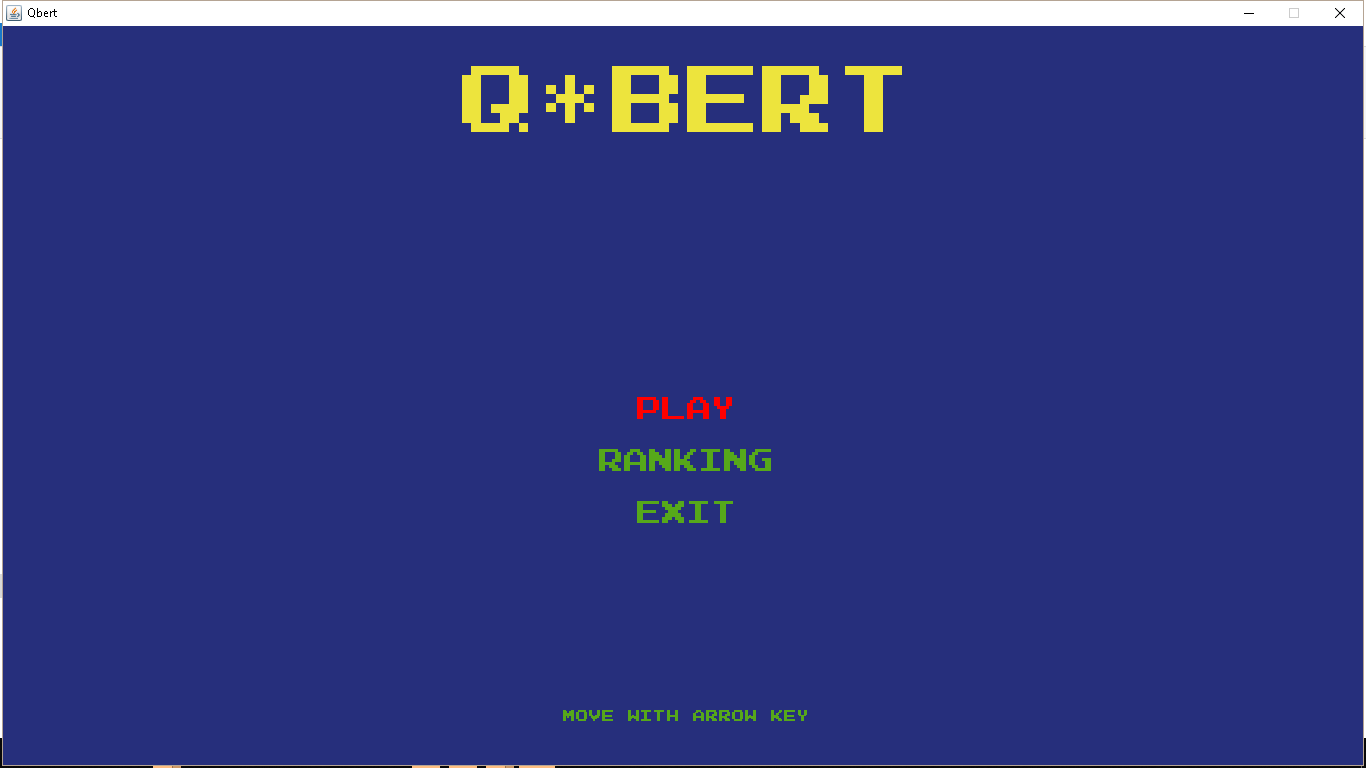
\includegraphics[width=\linewidth]{img/SchermataIniziale.png}
\label{img:SchermataIniziale}
\end{figure}

\subsubsection{Schermata di gioco}

\begin{figure}[H]
\centering{}
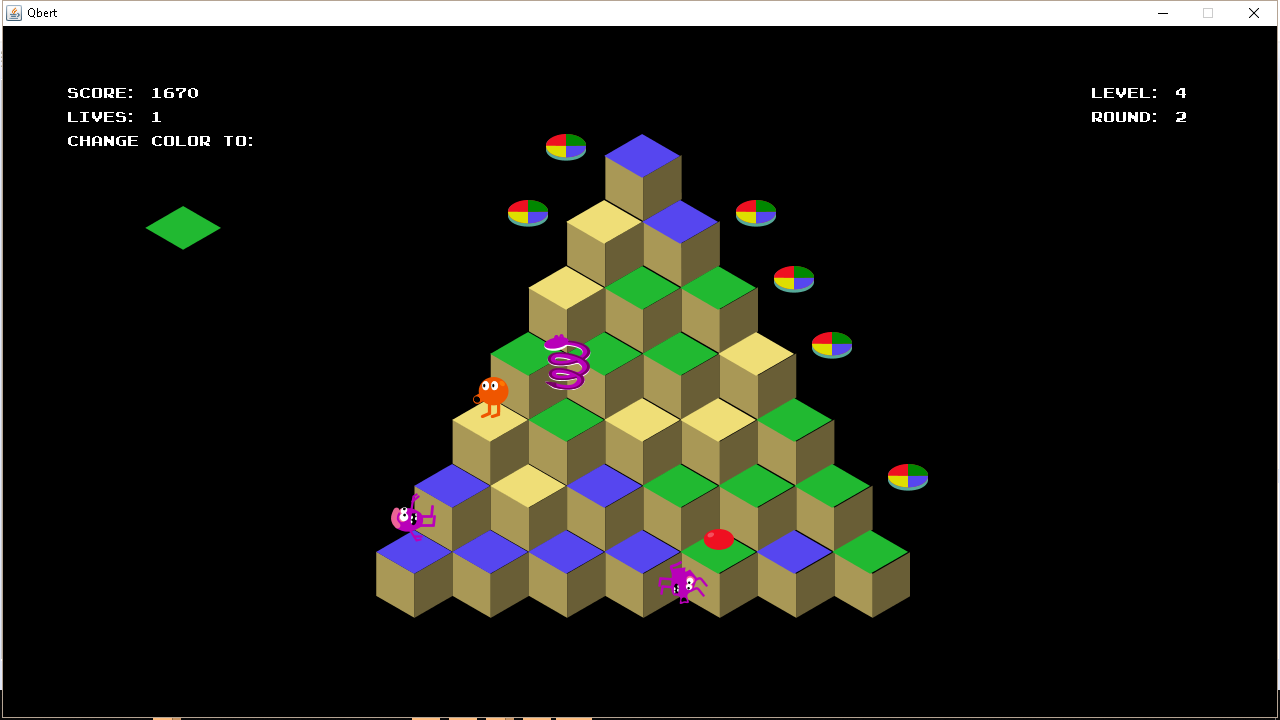
\includegraphics[width=\linewidth]{img/Gameplay.png}
\label{img:Gameplay}
\end{figure}

\subsubsection{Classifica}

\begin{figure}[H]
\centering{}
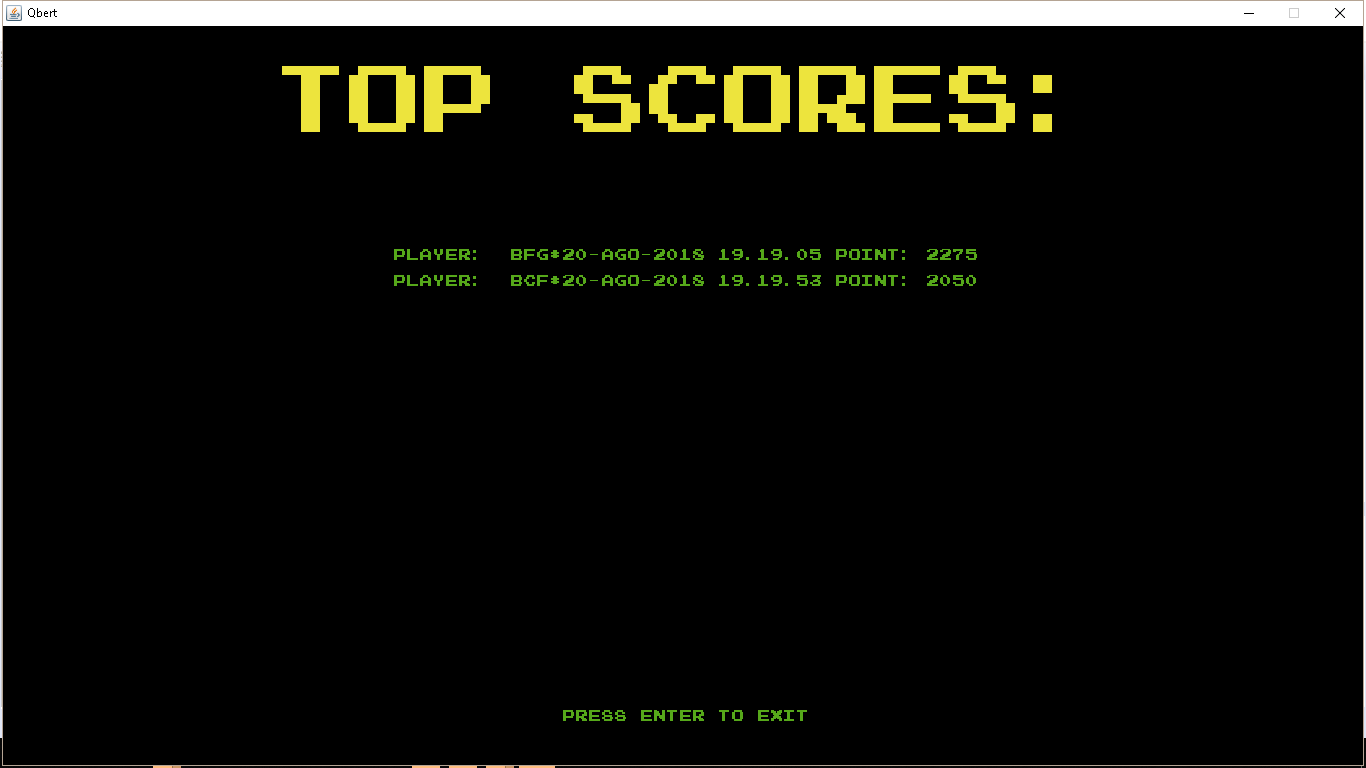
\includegraphics[width=\linewidth]{img/Classifica.png}
\label{img:Classifica}
\end{figure}

\subsubsection{Game Over}

\begin{figure}[H]
\centering{}
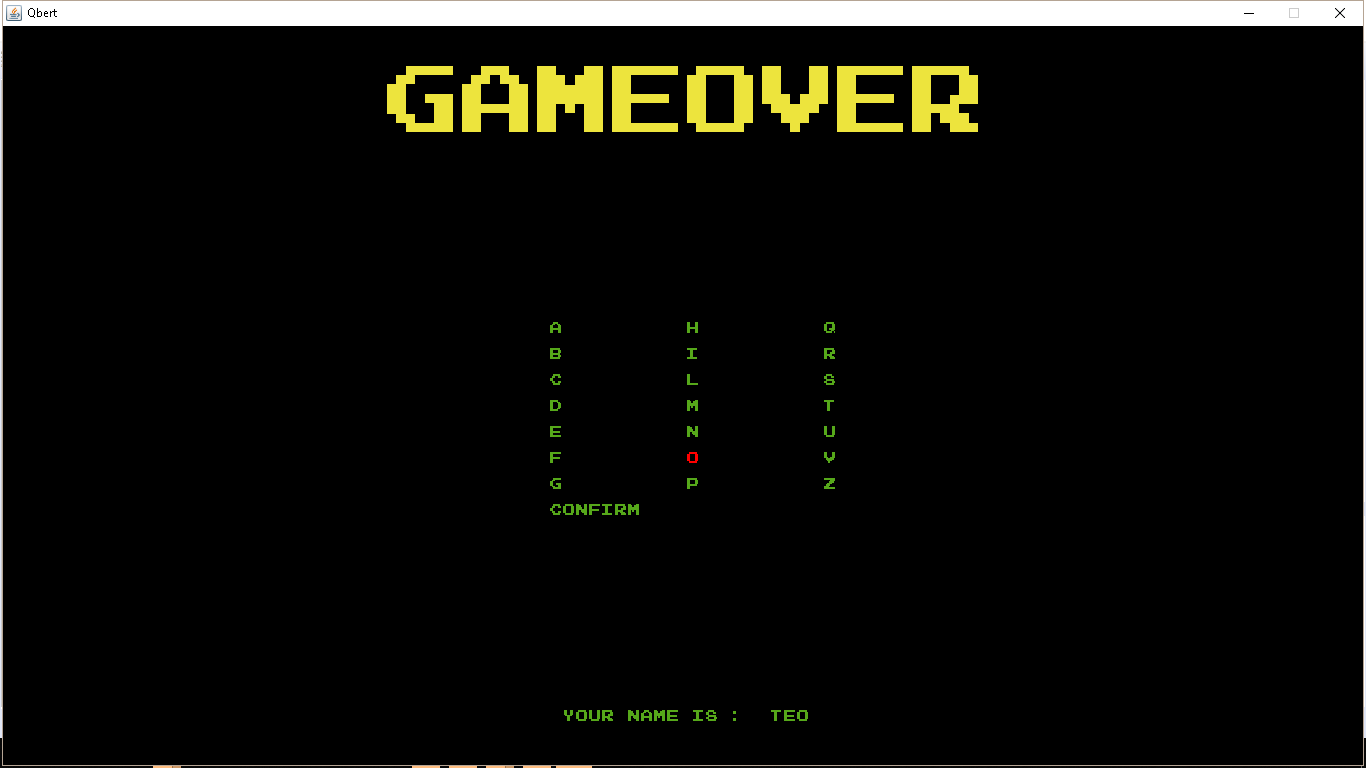
\includegraphics[width=\linewidth]{img/GameOver.png}
\label{img:GameOver}
\end{figure}

\chapter{Bibliografia}

\begin{itemize}
	\item Gamma E., Helm R., Johnson R., Vlissides J., \emph{Design Patterns. Elementi per il riuso di software a oggetti}, Milano, Pearson Paravia Bruno Mondadori, 2002, Prima edizione italiana.
	\item Robert Nystrom, \emph{Game Programming Patterns} \href{http://gameprogrammingpatterns.com/}{http://gameprogrammingpatterns.com/}
	\item \emph{Design Patterns. Explained Simply} \href{https://sourcemaking.com/design\_patterns}{https://sourcemaking.com/design\_patterns}

\end{itemize}

\end{document}
